\documentclass[11pt,a4paper]{article}
\usepackage[T1]{fontenc}
\usepackage[utf8]{inputenc}
\usepackage{lmodern,microtype}
\usepackage{amsmath,amssymb,amsthm,mathtools,bm}
\usepackage{booktabs,array,tabularx,longtable}
\usepackage{graphicx,float,caption}
\usepackage{xcolor}
\usepackage[margin=20mm]{geometry}
\usepackage{enumitem}
\usepackage{fancyhdr}
\usepackage[hidelinks]{hyperref}
\hypersetup{
  pdftitle={FIN ST46--ST57: Projective State, Carrier Transfer, and Entropy Boundaries},
  pdfauthor={Krzysztof Żuchowski},
  pdfsubject={Analytical and computational execution of FIN programs ST46--ST57},
  pdfkeywords={FIN, spectral operator, projective state, carrier invariance, entropy, refinement, symmetry breaking, falsification}
}
\setlength{\parindent}{0pt}
\setlength{\parskip}{0.50em}
\setlength{\emergencystretch}{2em}
\setlength{\headheight}{14pt}
\setlist[itemize]{leftmargin=1.55em,itemsep=0.16em,topsep=0.2em}
\setlist[enumerate]{leftmargin=1.75em,itemsep=0.16em,topsep=0.2em}
\pagestyle{fancy}
\fancyhf{}
\lhead{FIN ST46--ST57}
\rhead{Release 10.58}
\cfoot{\thepage}
\newtheorem{theorem}{Theorem}[section]
\newtheorem{proposition}[theorem]{Proposition}
\newtheorem{corollary}[theorem]{Corollary}
\newcommand{\proven}{\textcolor{green!40!black}{\textbf{[PROVEN]}}}
\newcommand{\strong}{\textcolor{blue!70!black}{\textbf{[STRONG EVIDENCE]}}}
\newcommand{\conditional}{\textcolor{black!60}{\textbf{[CONDITIONAL]}}}
\newcommand{\constructed}{\textcolor{violet!70!black}{\textbf{[CONSTRUCTED]}}}
\newcommand{\failed}{\textcolor{red!72!black}{\textbf{[REFUTED IN CLASS]}}}
\newcommand{\statusboundary}{\textcolor{orange!80!black}{\textbf{[BOUNDARY]}}}
\newcommand{\resultbox}[1]{\begin{center}\fcolorbox{blue!60!black}{blue!4}{\parbox{0.92\textwidth}{#1}}\end{center}}

\begin{document}

\pagenumbering{gobble}
\begin{titlepage}
\centering
\vspace*{1.25cm}
{\LARGE\bfseries FIN ST46--ST57\par}
\vspace{0.35cm}
{\Large Projective State, Carrier Transfer, and Entropy Boundaries\par}
\vspace{0.40cm}
{\large Upstream sensitivity, refinement selection, feedback nonidentifiability, projective holonomy, exact minimizers, and executable operational tests\par}
\vspace{1.05cm}
{\Large Krzysztof Żuchowski\par}
\vspace{0.24cm}
{\large Independent Researcher --- Fractal Information Theory Project\par}
{\large ORCID: 0009-0002-0909-3613\par}
\vspace{0.85cm}
{\large FIN Release 10.58 --- Version 1.0.0\par}
{\large August 10, 2026\par}
\vfill
\begin{minipage}{0.89\textwidth}
\textbf{Scope.} This report executes ST46--ST57, the next local analytical and computational batch after Release 10.57. It tests whether the earlier collision certificate survives upstream uncertainty, whether a scale law or fractal compression selects refinement, whether positive feedback is strict-sourced, and whether one enlarged projective state can package selector, algebra, and holonomy data. It also freezes a two-carrier transfer specification and audits the information-to-thermodynamics boundary.\par
\textbf{Method.} Directed interval evaluation of strict kernel entries, conservative perturbation bounds, exact finite-dimensional algebra, rational root isolation, deterministic simulations, synthetic preregistration, explicit counterfamilies, and seventeen live acceptance tests.\par
\textbf{Epistemic rule.} A theorem is reported only in its declared finite model or construction class. Conditional objects are not treated as strict consequences. Local synthetic receivers are not laboratory evidence.\par
\textbf{Repository snapshot.} Git commit \texttt{ac8d649f4f262abd010abe4546a51ae893ce5926}; the working tree contained additional local research artifacts and is recorded by the release manifest.\par
\textbf{Repository.} \url{https://github.com/hyconiek/Fractal-Nadsoliton-Theory}\par
\textbf{License.} CC BY 4.0.
\end{minipage}
\end{titlepage}
\pagenumbering{arabic}

\begin{abstract}
This report closes twelve local programs. ST46 propagates interval-regenerated strict-kernel uncertainty through the hidden-memory construction and the collision calculation. It confines the collision speed to
\[
1.2780147516944267\le s_*\le1.2780147519464700,
\]
but remains a strong partial certificate because the projector, memory, inverse, and root inequalities are evaluated in binary64 with a conservative factor-16 payment rather than by one all-directed interval computation.

ST47 proves that trace-density conservation uniquely selects the zero-fine-weight dyadic lift, while also proving why this is conditional: a different prescribed scaling multiplier selects a different lift. ST56 strengthens the obstruction. Every coarse-intertwining loss vanishes on the entire tested lift fibre, and three directed interval ratios $K(2d)/K(d)$ are pairwise disjoint, excluding one exact dyadic amplitude ratio for $d=1,2,3$. Fractal compression therefore remains a research premise until a fine-data-retaining code and objective are derived.

ST48 gives the batch's principal negative theorem. The same strict operator and reflection symmetry admit equivariant adaptive potentials with negative, zero, or positive odd-sector gain while keeping the strict operator stationary. Positive feedback is therefore not identified by the static strict core. ST49 gives the principal constructive result: a two-component real projective half-angle texture has Pancharatnam holonomy $-1$, and distinct amplitudes make its density generate $M_{12}(\mathbb C)$ together with the connected strict operator. This single enlarged state type can carry selector data, full algebra, and $\pi$ holonomy, but the texture and amplitude order were inserted. It does not discharge QW-2191 or select chirality.

ST50 classifies finite linear intertwiners among unitary, heat, wave, Green, and Gibbs spectral images. Shared dependence on $A$ does not make different channels dynamically similar. ST51 obtains perfect synthetic mismatch power and a $0.00333$ hold-out false-rejection rate at the frozen receiver, while ST55 exports a hashed executable specification. Both carriers, clocks, detectors, events, and custody remain simulated.

ST52 exactly identifies the global minimizers of the constructed saturating DNLS model as one uniform $U(1)$ orbit and proves orbital stability; this is a rigorous nonlocalization result, not a particle derivation. ST53 proves Shannon increase and relative-entropy contraction for the strict heat kernel, unitary invariance of von Neumann entropy, and non-affinity of normalized amplitude heat filtering. It also isolates the missing thermodynamic bridge: bath, energy scale, and temperature are not supplied by dimensionless information entropy. ST54 states the universal property of carrier-neutral operational equivalence. ST57 finds that conditional packaging has not reduced the nine independent source groups required for physical completion.
\end{abstract}

\textbf{Status vocabulary.} \proven{} denotes an analytic or exact finite result in the declared model. \strong{} denotes robust but not fully interval-certified numerical evidence. \conditional{} denotes a theorem after named extra premises. \constructed{} denotes a complete object or protocol whose physical origin is not derived. \failed{} means a proposed strict implication is destroyed by a counterexample in its declared class. \statusboundary{} states the exact non-implication.

\tableofcontents
\newpage

\section{Starting object, questions, and kernel discipline}

The strict finite working operator is
\begin{equation}
W_{xx}=0,\qquad
W_{xy}=\frac{\cos(0.18575d(x,y)+0.16250)}{1+d(x,y)^{1.8}}\quad(x\ne y),
\qquad A=sI-W,
\label{eq:strict}
\end{equation}
on the cycle $C_{12}$, where $d$ is cycle distance and $s=\sum_{y\ne x}W_{xy}=1.6603072787660986$ to the displayed precision. Hence
\[
\langle f,Af\rangle=\frac12\sum_{x,y}W_{xy}|f_x-f_y|^2\ge0.
\]
All strict weights on $C_{12}$ are positive. The zero diagonal in~\eqref{eq:strict} is part of the definition; evaluating the scalar profile at $d=0$ would create a different operator.

No step in this batch silently transfers the historical physical roles of the intermediate legacy kernel to $K_{\mathrm{strict}}$. No legacy-to-strict completion theorem, dimensional calibration, Standard Model sector, gravity law, or Theory-of-Everything closure is claimed.

The batch addresses four linked questions:
\begin{enumerate}
\item Does the earlier stability collision survive uncertainty propagated from the strict transcendental kernel?
\item Can refinement, fractal compression, or symmetry determine the missing scale and positive-feedback choices?
\item Can an enlarged state type jointly encode selection, a full observable algebra, and nontrivial holonomy?
\item What exactly survives a change of carrier, and where does information stop short of thermodynamics?
\end{enumerate}

\resultbox{\textbf{Central result.} The projective state construction shows that several missing formal roles can be \emph{packaged} by one enlarged object, but ST48 and ST57 show that the package is not generated by the strict operator. Current FIN therefore has a mathematically coherent core and useful conditional completions, but no strict source theorem for feedback, realized state, scale, or physical carrier.}

\section{Outcome matrix}

\small
\begin{longtable}{@{}p{0.055\textwidth}p{0.30\textwidth}p{0.22\textwidth}p{0.35\textwidth}@{}}
\toprule
ID & Object & Outcome & Exact boundary\\
\midrule
\endfirsthead
\toprule
ID & Object & Outcome & Exact boundary\\
\midrule
\endhead
ST46 & Upstream strict-to-memory certificate & \strong{} & Not an all-directed interval replay\\
ST47 & Trace-stationary refinement & \conditional{} unique $q=0$ & Scale law is added\\
ST48 & Odd-gain source test & \proven{} no-identification & Counterfamily does not choose dynamics\\
ST49 & Projective selector-holonomy state & \conditional{} joint package & State texture and ordering inserted\\
ST50 & Channel intertwiner classification & \proven{} & Parameter-specific finite classification\\
ST51 & Finite-count carrier transfer & \strong{} synthetic & No laboratory carriers or external custody\\
ST52 & Saturating DNLS minimizer orbit & \proven{} uniform stability & Saturation added; localization fails\\
ST53 & Entropy/data-processing ledger & \proven{} & No bath, temperature, or energy scale\\
ST54 & Operational quotient & \proven{} universal property & Classification, not physical realization\\
ST55 & Executable transfer specification & \constructed{} & File roles are not independent custody\\
ST56 & Compression/refinement audit & \proven{} nonselection & Richer sourced fractal code remains open\\
ST57 & Minimal-axiom reconciliation & \proven{} relative no-reduction & Relative to current targets and classes\\
\bottomrule
\end{longtable}
\normalsize

\section{ST46 --- Upstream strict-to-memory sensitivity}

The earlier collision calculation used a reduced hidden-memory representation. ST46 begins instead from directed intervals for the exact decimal inputs
\[
\omega=\frac{743}{4000},\qquad \phi=\frac{13}{80},\qquad \eta=\frac95,\qquad \beta=1,
\]
and regenerates the strict matrix interval. The induced operator-norm input radius, after the factor-16 arithmetic payment, is
\[
\delta_A\le1.2351231148954867\times10^{-14}.
\]

The hidden block has four spectral clusters. If $P_j$ is a cluster projector, $p_j$ its pole, and $r_j$ its residue, Davis--Kahan-type gap bounds and resolvent identities give conservative enclosures for
\[
M=F(0)I-\sum_j r_j(A+p_jI)^{-1}.
\]
The memory error is bounded by $4.714644761817467\times10^{-13}$ and the combined operator error by
\[
\delta_{A+M}\le4.838157073307016\times10^{-13}.
\]

For the stationary equation
\[
(A+M)u+u-u^{\circ3}=0,
\]
the center residual is $4.93\times10^{-16}$. The inverse-Newton image is strictly included in all tested Euclidean balls from radius $10^{-12}$ through $10^{-8}$. The first accepted radius is $10^{-12}$.

The collision polynomial in $x=s^{-1}$ is
\[
p(x)=ax^2+bx+c,
\]
with propagated coefficient intervals
\begin{align*}
0.2671565201170468&\le a\le0.2671565201202012,\\
0.11221794517447314&\le b\le0.11221794519510192,\\
-0.2513728361412824&\le c\le-0.25137283607752287.
\end{align*}
Monotone endpoint evaluation then yields the stated collision interval.

\begin{figure}[H]
\centering
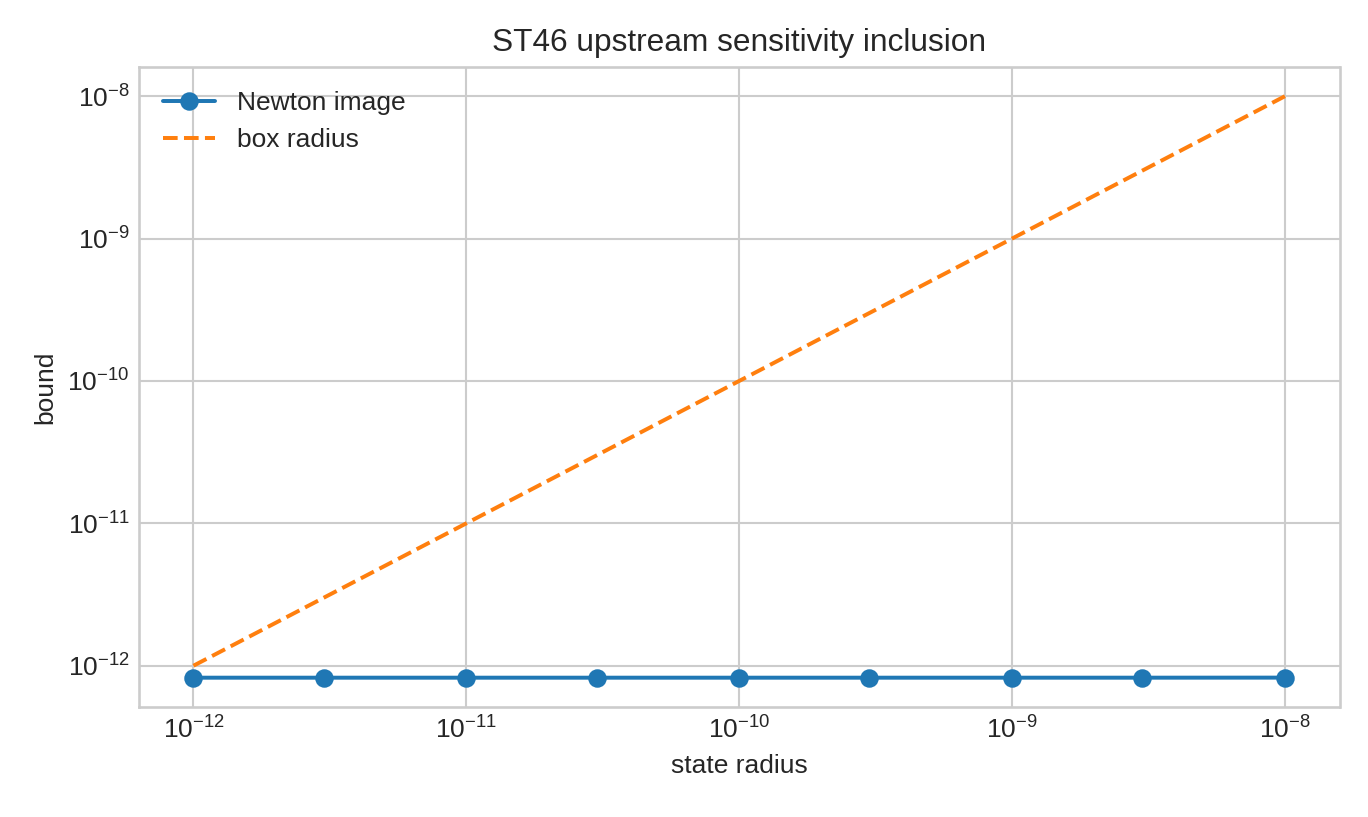
\includegraphics[width=0.92\textwidth]{FIN_ST46_ST57_Figures/st46_upstream_sensitivity.png}
\caption{ST46 upstream sensitivity. The left panel records spectral cluster gaps and residue bounds; the right panel records strict inverse-Newton inclusions.}
\end{figure}

\statusboundary{} This is deliberately not labelled a full proof certificate. Directed intervals cover the strict transcendental input, but spectral projectors, memory resolvents, inverses, and final root propagation are analytic perturbation bounds evaluated in binary64 with a factor-16 safety multiplier. ST58 must replay the whole chain in one outward-rounded system or proof assistant.

\section{ST47 and ST56 --- Refinement and fractal-compression nonselection}

Let $J:\mathbb C^{12}\rightarrow\mathbb C^{24}$ be the periodic coarse embedding and $A_{24}(q)$ the ST18 dyadic lift. Every $q\ge0$ satisfies
\[
A_{24}(q)J=JA_{12}.
\]
Thus coarse intertwining alone cannot choose the fine operator.

\subsection{A conditional trace selector}

Direct block tracing gives the exact identity
\begin{equation}
\frac{\operatorname{tr}A_{24}(q)}{24}
=\frac{\operatorname{tr}A_{12}}{12}+q.
\label{eq:trace-refinement}
\end{equation}
Consequently, exact trace-density conservation selects $q=0$ uniquely. More generally, imposing
\[
\frac{\operatorname{tr}A_{24}(q)}{24}=c\frac{\operatorname{tr}A_{12}}{12}
\]
selects $q=(c-1)s_{12}$. For $c=1.05$ and $1.20$ the selected values are $0.08301536$ and $0.33206146$, respectively.

\begin{theorem}[Conditional refinement selection]
Within the ST18 lift family, trace-density conservation uniquely selects $q=0$. The selection is supplied by the added scale law and not by the coarse intertwining equation.
\end{theorem}

\subsection{Why coarse compression is insufficient}

Any objective depending only on
\[
\mathcal L_{\rm coarse}(q)=\|A_{24}(q)J-JA_{12}\|_F^2
\]
is constant on the full $q\ge0$ fibre. The computed losses remain below $2.9\times10^{-30}$ for $q=0,0.1,0.3,0.9$. Adding $q^2$ selects $q=0$, but the choice and coefficient of that complexity penalty are new assumptions.

The strict profile also fails a simpler exact self-similar test. Directed interval arithmetic gives
\begin{align*}
\frac{K(2)}{K(1)}&\in[0.40861575760236660,0.40861575760236674],\\
\frac{K(4)}{K(2)}&\in[0.24488803884204619,0.24488803884204624],\\
\frac{K(6)}{K(3)}&\in[0.12108700770405440,0.12108700770405442].
\end{align*}
These intervals are pairwise disjoint. The corresponding effective powers range from $1.29118$ to $3.04588$.

\begin{theorem}[Declared compression nonselection]
The coarse reconstruction criterion cannot select a dyadic lift, and the strict profile has no single exact dyadic amplitude ratio over $d=1,2,3$. Therefore neither tested notion supplies a strict-sourced fractal refinement law.
\end{theorem}

\begin{figure}[H]
\centering
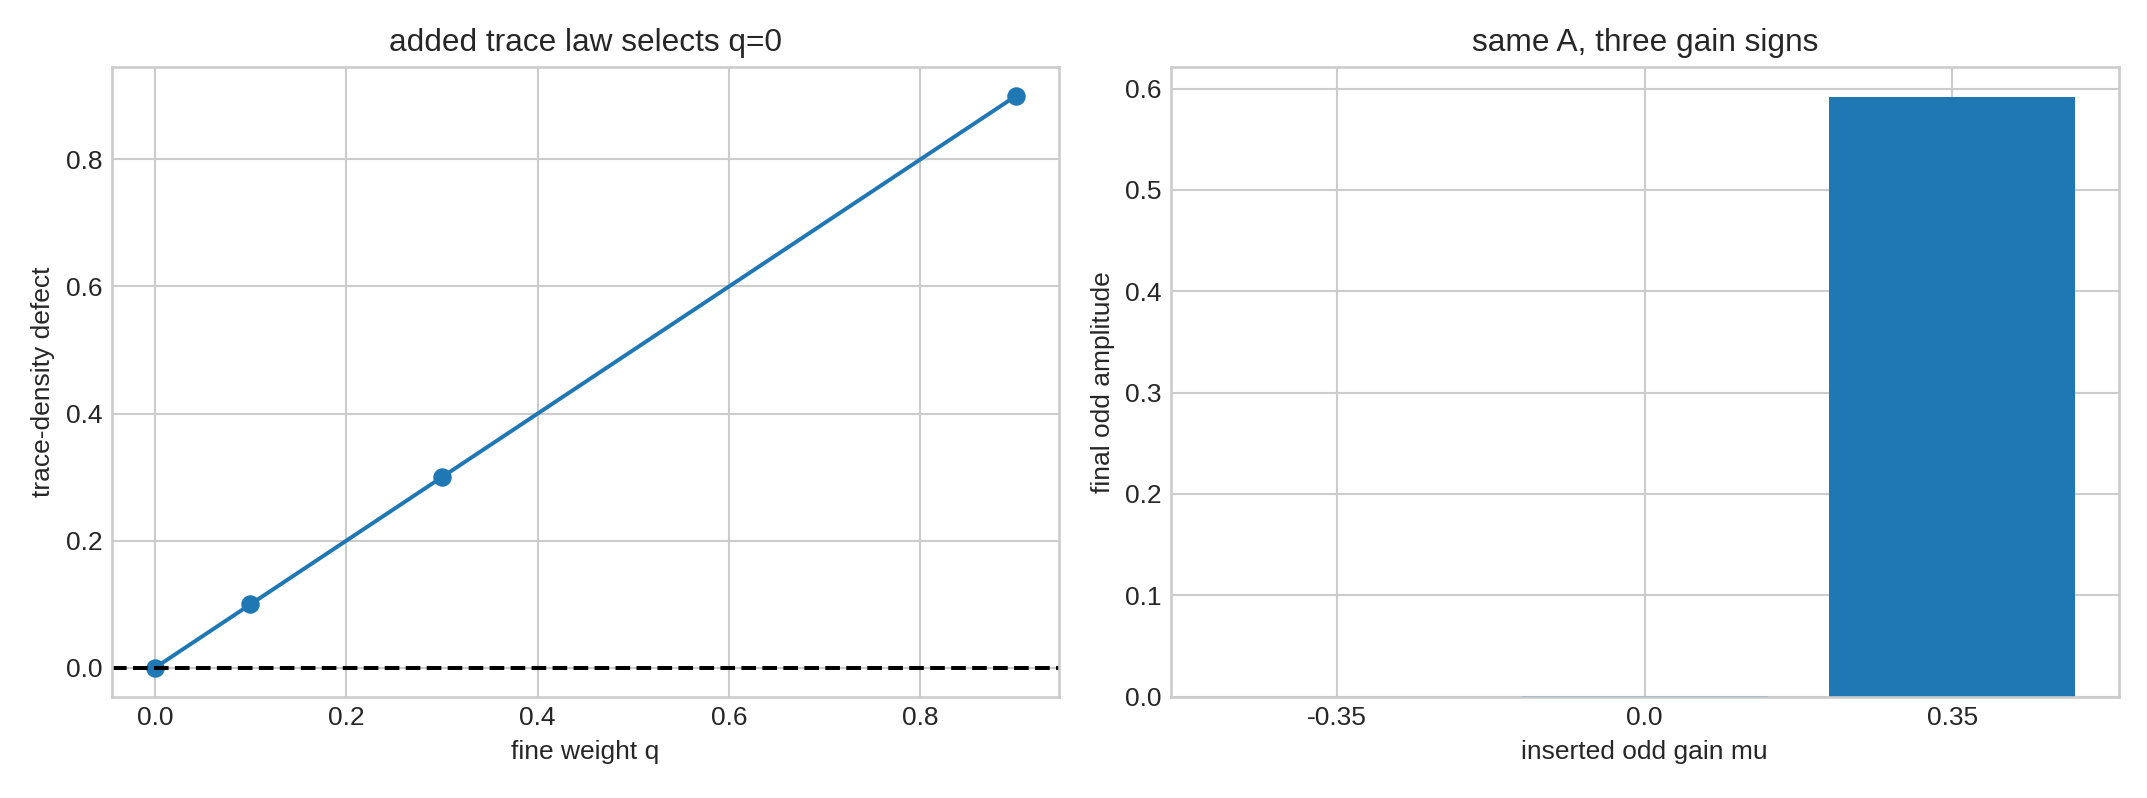
\includegraphics[width=0.96\textwidth]{FIN_ST46_ST57_Figures/st47_refinement_st48_gain.png}
\caption{Left: a trace law can select one lift, but changing the law changes the selected $q$. Right: the strict stationary point is compatible with all three feedback-gain signs.}
\end{figure}

\statusboundary{} This does not refute fractal compression in general. It refutes selection by the declared coarse loss and by a single exact dyadic profile ratio. A successful future code must retain fine data, define a sourced distortion or rate functional, and prove why its objective is physically operative.

\section{ST48 --- Positive feedback is not strict-sourced}

Let $R$ be reflection and let $P_-$ and $P_+$ project operator perturbations onto reflection-odd and reflection-even sectors. Consider the equivariant potential family around the same strict fixed operator:
\begin{equation}
\mathcal F_\mu(A+H)=
-\frac{\mu}{2}\|P_-H\|_F^2
+\frac14\|P_-H\|_F^4
+\frac12\|P_+H\|_F^2.
\label{eq:gain-family}
\end{equation}
For every real $\mu$, $H=0$ is stationary and the functional respects the same reflection symmetry. Along a normalized odd direction $H=xH_-$, gradient descent reduces to
\[
\dot x=\mu x-x^3.
\]
Thus $\mu<0$ damps, $\mu=0$ is marginal at linear order, and $\mu>0$ amplifies before saturation.

\begin{theorem}[Odd-gain nonidentifiability]
The strict static operator $A$ and its reflection stabilizer do not determine the sign of odd-sector adaptive gain. Any claim of positive self-coupling requires a response functional, state law, or equivalent additional premise.
\end{theorem}

The deterministic trajectories from $x(0)=10^{-4}$ end at approximately $8.1\times10^{-11}$, $10^{-4}$, and $0.59160$ for $\mu=-0.35,0,+0.35$. These trajectories illustrate the analytic counterfamily; they are not the proof.

\statusboundary{} Symmetry supplies equivalent directions and permits an instability, but does not itself provide amplification. Equation~\eqref{eq:gain-family} destroys the inference ``strict symmetry implies positive feedback'' while leaving open a future theorem that derives one particular response law from a genuinely new state-dependent object.

\section{ST49 --- A projective state that packages three missing roles}

ST38 left open multi-component and projective constructions. ST49 introduces real two-component rays
\[
r_x=\begin{pmatrix}
\cos(\theta_x/2)\\ \sin(\theta_x/2)
\end{pmatrix},\qquad \theta_x=\frac{2\pi x}{12},\qquad x=0,\ldots,11.
\]
Although $\theta$ completes one turn, the half-angle representative changes sign. The gauge-invariant Pancharatnam product is
\[
\mathcal H=\prod_{x=0}^{11}
\frac{\langle r_x,r_{x+1}\rangle}{|\langle r_x,r_{x+1}\rangle|}=-1,
\]
so the projective flux is $\pi$. Its cyclic-shift residual is below $5.6\times10^{-16}$.

Now choose amplitudes $a_x=1+0.02x$ and define $\psi_x=a_xr_x$. The normalized density has one maximum. Its dihedral orbit has 24 members. Because all diagonal entries of $D_\psi=\operatorname{diag}\|\psi_x\|^2$ are distinct and the support graph of $A$ is connected, every matrix commuting with both $A$ and $D_\psi$ is scalar. The finite bicommutant theorem gives
\[
C^*(A,D_\psi)=M_{12}(\mathbb C),\qquad \dim=144.
\]

\begin{proposition}[Conditional joint package]
A two-component projective state can simultaneously carry a density selector, the full matrix algebra, and nontrivial $\pi$ holonomy. This is impossible for the one-component phase-gradient class tested in ST38 but possible after enlarging the state type.
\end{proposition}

\begin{figure}[H]
\centering
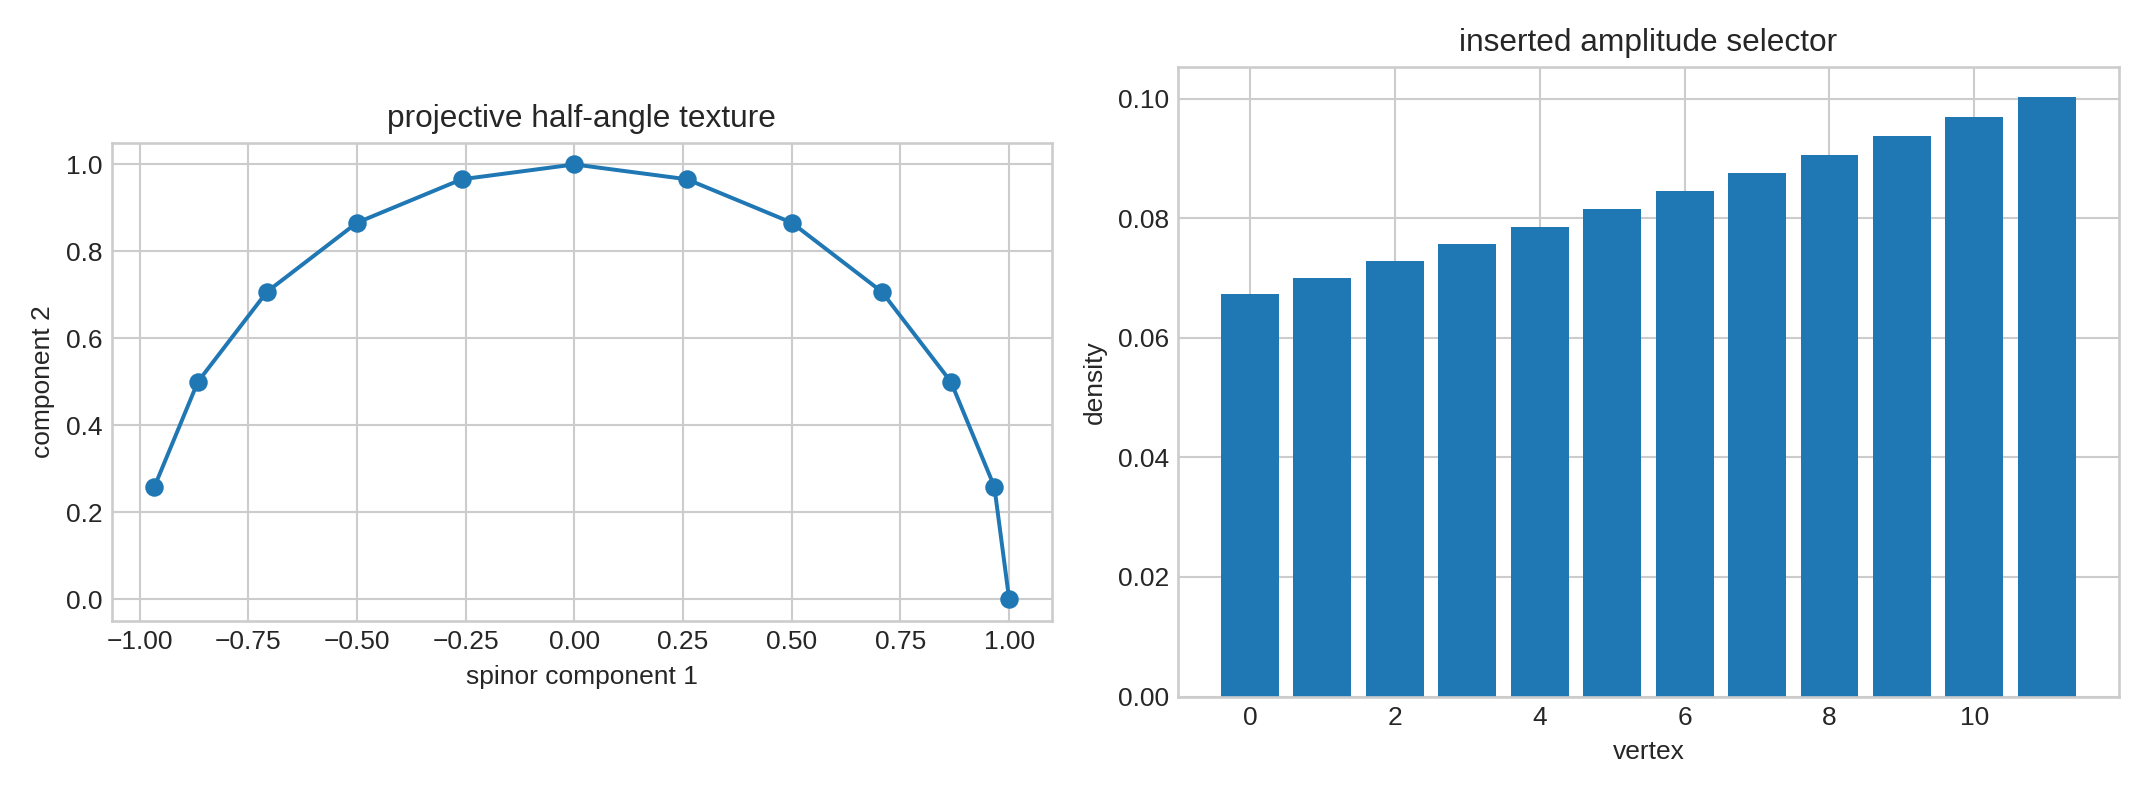
\includegraphics[width=0.92\textwidth]{FIN_ST46_ST57_Figures/st49_projective_state.png}
\caption{The inserted projective half-angle texture and its distinct density amplitudes. The state packages several formal obligations but is not generated by the strict operator.}
\end{figure}

\statusboundary{} This is a conditional existence theorem, not selector closure. The ordered amplitudes and projective texture were inserted. Reflection maps the $\pi$ sector to itself, so $\pi$ flux does not select chirality. No canonical origin is obtained. QW-2191 remains open.

\section{ST50 --- Common spectrum does not imply common dynamics}

For the seven distinct strict eigenvalues, consider
\[
f_U(\lambda)=e^{-it\lambda},\quad
f_H(\lambda)=e^{-\tau\lambda},\quad
f_C(\lambda)=\cos(t\sqrt\lambda),\quad
f_G(\lambda)=\frac1{\lambda+z},
\]
and normalized Gibbs weights $f_\beta(\lambda)=e^{-\beta\lambda}/Z$. The frozen parameters are $t=\tau=0.61$, $z=1$, and $\beta=0.8$.

If $F=f(A)$ and $G=g(A)$ are normal, the solutions of $FX=XG$ are mode-pair blocks for which $f(\lambda_i)=g(\lambda_j)$. Hence
\[
\dim\operatorname{Int}(F,G)=
\sum_{\alpha=\gamma}\dim E^F_\alpha\dim E^G_\gamma.
\]
Each self-intertwiner space has dimension 22 because of the $C_{12}$ spectral multiplicities. Each cross-pair among unitary, heat, wave, and Green has dimension one, arising only from their shared zero-mode value $1$. Gibbs cross-intertwiner dimensions are zero under the normalized weighting. No cross-channel pair has an invertible intertwiner.

\begin{theorem}[Finite channel inequivalence]
At the declared parameters, the five spectral images are injective on the seven distinct strict eigenvalues, yet no two different channels are similar. Sharing the source operator does not make their dynamics operationally interchangeable.
\end{theorem}

\begin{figure}[H]
\centering
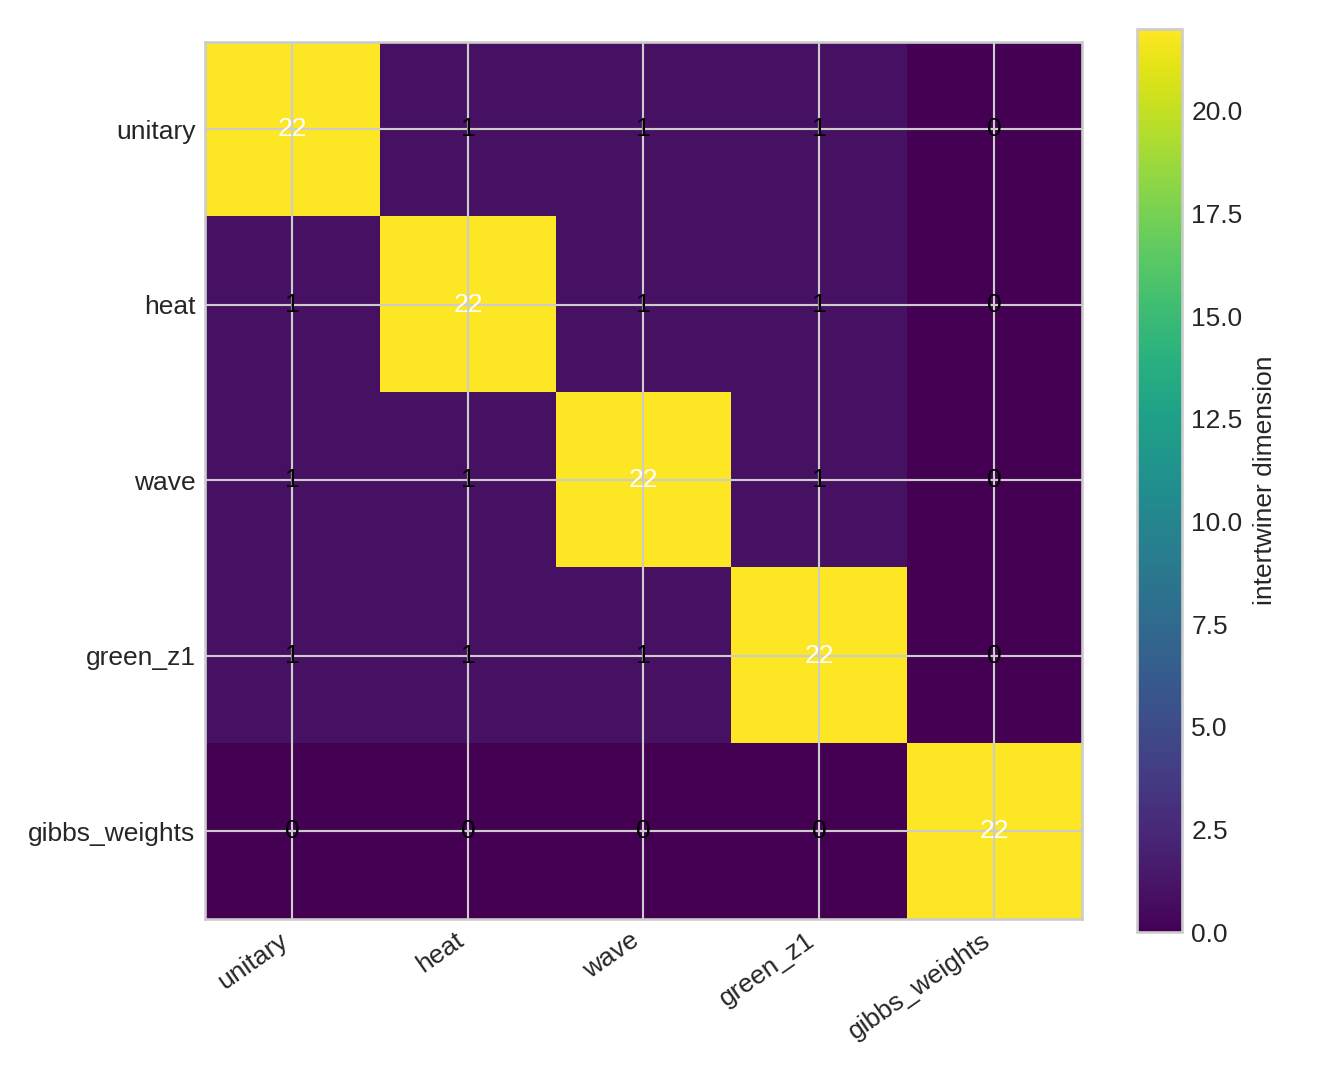
\includegraphics[width=0.78\textwidth]{FIN_ST46_ST57_Figures/st50_channel_intertwiners.png}
\caption{Dimensions of the five-by-five linear intertwiner table. The diagonal value 22 records spectral multiplicities; sparse cross-intertwiners do not yield channel equivalence.}
\end{figure}

\statusboundary{} Gibbs weights are a state spectrum, not a time-evolution channel. The table is an exact finite classification after the displayed parameter values are fixed; it is not a claim that actual wave, diffusive, thermal, and quantum media instantiate one FIN process.

\section{ST51 and ST55 --- A frozen two-carrier transfer test}

ST51 specializes the operational-carrier theorem from Release 10.57. Carrier A uses vertex preparations and effects. Carrier B uses a dense orthogonal $Q$ fixing the uniform mode:
\[
A_B=QAQ^T,\qquad \rho_x^B=Q\rho_x^AQ^T,
\qquad E_y^B=QE_y^AQ^T.
\]
Complete transport preserves every registered probability to $1.55\times10^{-15}$. Transporting $A$ while leaving preparations and measurements untransported creates mean total variation $0.14414$.

The preregistered synthetic receiver uses 12 preparations, 12 outcomes, 1,200 shots per preparation, dimensionless time $0.63$, 300 training-null trials, 300 frozen hold-out trials, and 300 mismatch trials. The 0.99 training quantile fixes the Pearson threshold at $198.2152$. Results are
\[
\widehat\alpha=0.003333,\qquad \widehat{\rm power}=1.000.
\]

\begin{figure}[H]
\centering
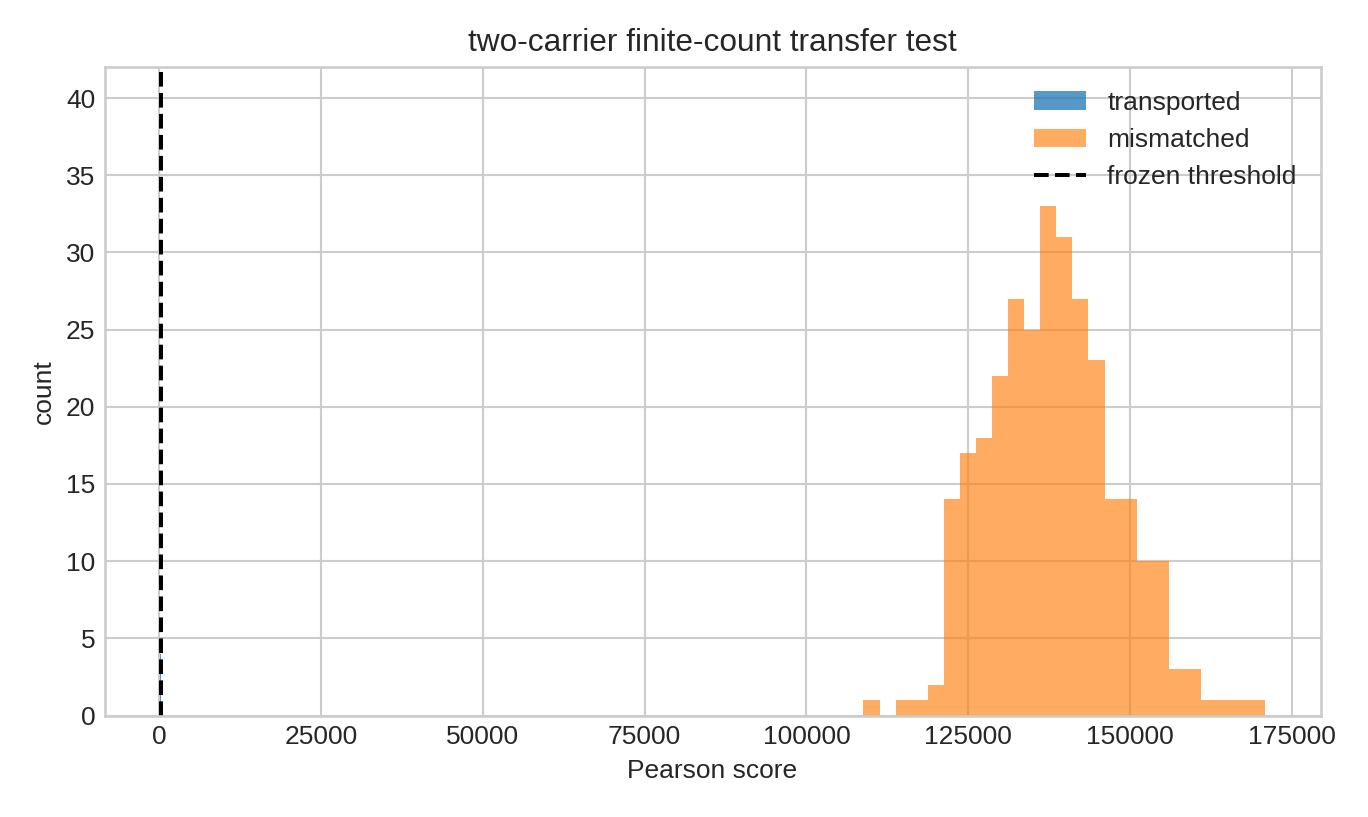
\includegraphics[width=0.92\textwidth]{FIN_ST46_ST57_Figures/st51_two_carrier_test.png}
\caption{Frozen synthetic score distributions. The separation tests the declared mismatch, not FIN against physical data.}
\end{figure}

ST55 exports the experiment as a hashed executable specification. Its raw event schema contains
\[
(\texttt{timestamp},\texttt{carrier\_id},\texttt{preparation\_id},
\texttt{outcome\_id},\texttt{run\_id},\texttt{calibration\_split},
\texttt{blind\_label}).
\]
The provider, registrar, analyst, and custodian are logically distinct roles. The document freezes a one-run rule and prohibits refitting $Q$, time, effects, threshold, or kernel after failure. The specification hash is
\[
\texttt{70e4bcf50bacff312c2089ccd0b3287bd79ca044689c5c916c2d26e21826bfb4}.
\]

\statusboundary{} Synthetic carriers are not laboratory platforms. A JSON role field cannot create independent custody, physical calibration, apparatus, or raw external events. The protocol is executable locally and transferable to a laboratory team, but has not been executed in a laboratory.

\section{ST52 --- Exact uniform minimizer and nonlocalization}

For the constructed ST34 saturation, the onsite potential is
\[
V(\rho)=-\frac12\left(\frac{\rho}{1+\rho/2}\right)^2+\frac{0.15}{2}\rho.
\]
Writing $y=1+\rho/2$, the sign of $V'(\rho)$ is the sign of
\[
3y^3-80y+80.
\]
Exact rational bisection isolates the smaller positive critical point at $y\simeq1.0424855672$ and the unique global onsite minimum at
\[
y_*=4.563202569446899,qquad
\rho_*=7.126405138893798,qquad |\psi|=2.669532756662446.
\]

Because $A$ is a connected positive-weight graph Laplacian, its Dirichlet energy is nonnegative and vanishes exactly on constant vectors. Therefore the complete global minimizer set is
\[
\mathcal M=\{\sqrt{\rho_*}e^{i\theta}\mathbf 1:\theta\in S^1\}.
\]
The radial curvature is $0.40277$. The phase Hessian has one $U(1)$ zero mode and positive gap $0.75412$.

\begin{theorem}[Constructed saturation minimizers]
The global minimizers of the declared saturating DNLS energy are exactly the uniform $U(1)$ orbit, and this orbit is stable modulo global phase.
\end{theorem}

\begin{figure}[H]
\centering
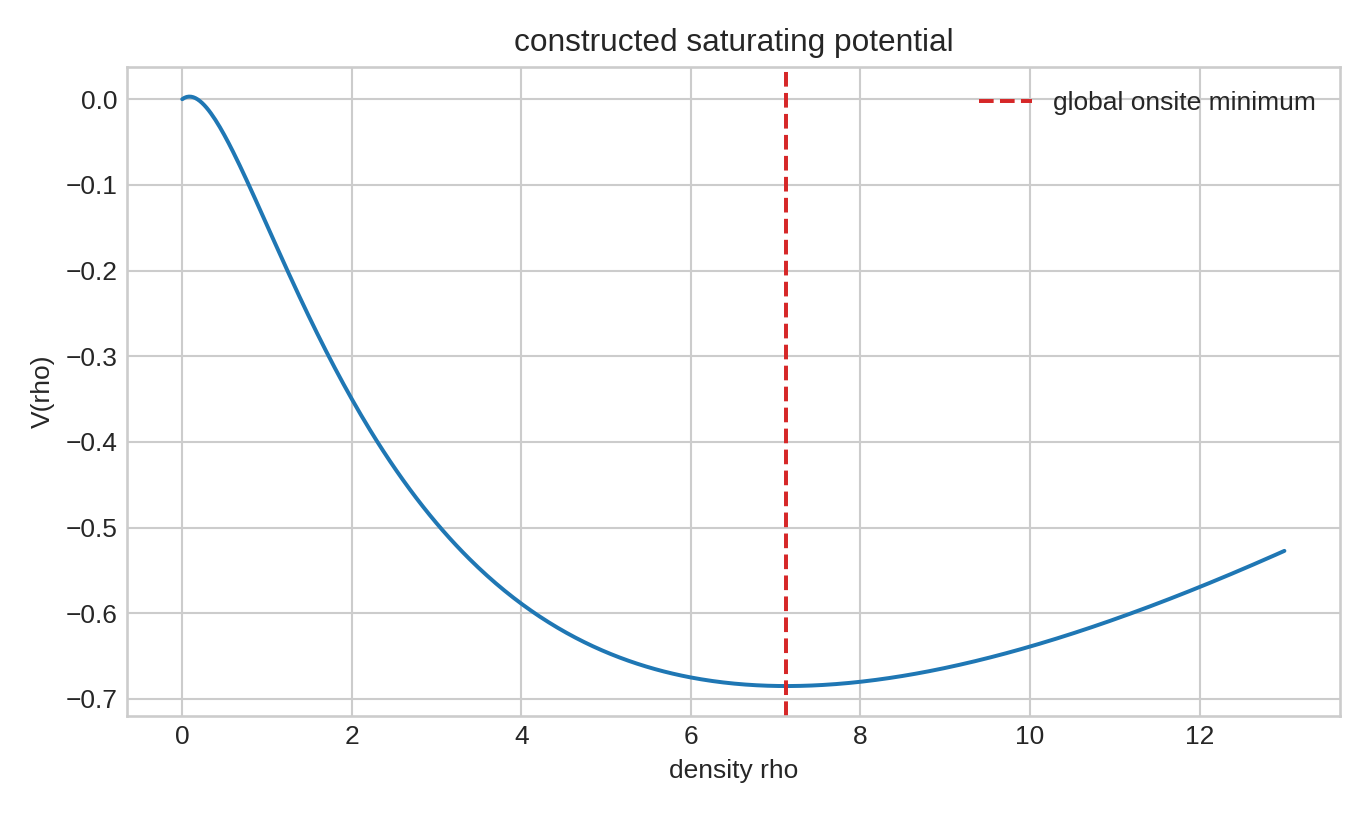
\includegraphics[width=0.84\textwidth]{FIN_ST46_ST57_Figures/st52_uniform_minimizer.png}
\caption{The exact onsite critical structure and the resulting uniform minimizer density.}
\end{figure}

\statusboundary{} This closes the constructed variational model but gives a rigorous negative answer to the intended localization question: its ground state is not a localized soliton. The saturation and coefficient $0.15$ are additional laws, not strict-derived physics.

\section{ST53 and ST54 --- Information invariants and their boundary}

Since $A$ is a positive connected graph Laplacian, $P_\tau=e^{-\tau A}$ has strictly positive entries and is doubly stochastic. At $\tau=0.4$ its smallest entry is $0.00804616$ and its row and column residuals are below $2.3\times10^{-16}$. Consequently,
\[
H(P_\tau p)\ge H(p),\qquad
D(P_\tau p\|P_\tau q)\le D(p\|q).
\]
For the frozen distributions,
\[
H:2.32750\longrightarrow2.42274,
\qquad D:0.67194\longrightarrow0.24411.
\]
Unitary conjugation preserves von Neumann entropy to $8.9\times10^{-16}$.

A frequently tempting map is the normalized amplitude filter
\[
\Phi_\tau(\rho)=
\frac{e^{-\tau A}\rho e^{-\tau A}}{\operatorname{tr}(e^{-\tau A}\rho e^{-\tau A})}.
\]
Its affinity defect on the declared state pair is $0.31095$. Hence it is nonlinear and cannot be silently treated as a completely positive trace-preserving channel.

\begin{theorem}[Finite information ledger]
The strict heat kernel supplies a classical doubly stochastic data-processing map, and strict unitary evolution preserves quantum entropy. Neither result converts dimensionless information entropy into thermodynamic entropy.
\end{theorem}

ST54 formalizes carrier-neutrality. Let $\mathrm{Rep}_{\rm op}$ be the groupoid of finite operational realizations and their operational isomorphisms. The quotient
\[
\pi:\mathrm{Rep}_{\rm op}\to\pi_0(\mathrm{Rep}_{\rm op})
\]
has the universal property that every isomorphism-invariant set-valued map factors uniquely through $\pi_0$. The proof is the well-defined assignment $\bar F([R])=F(R)$.

\begin{figure}[H]
\centering
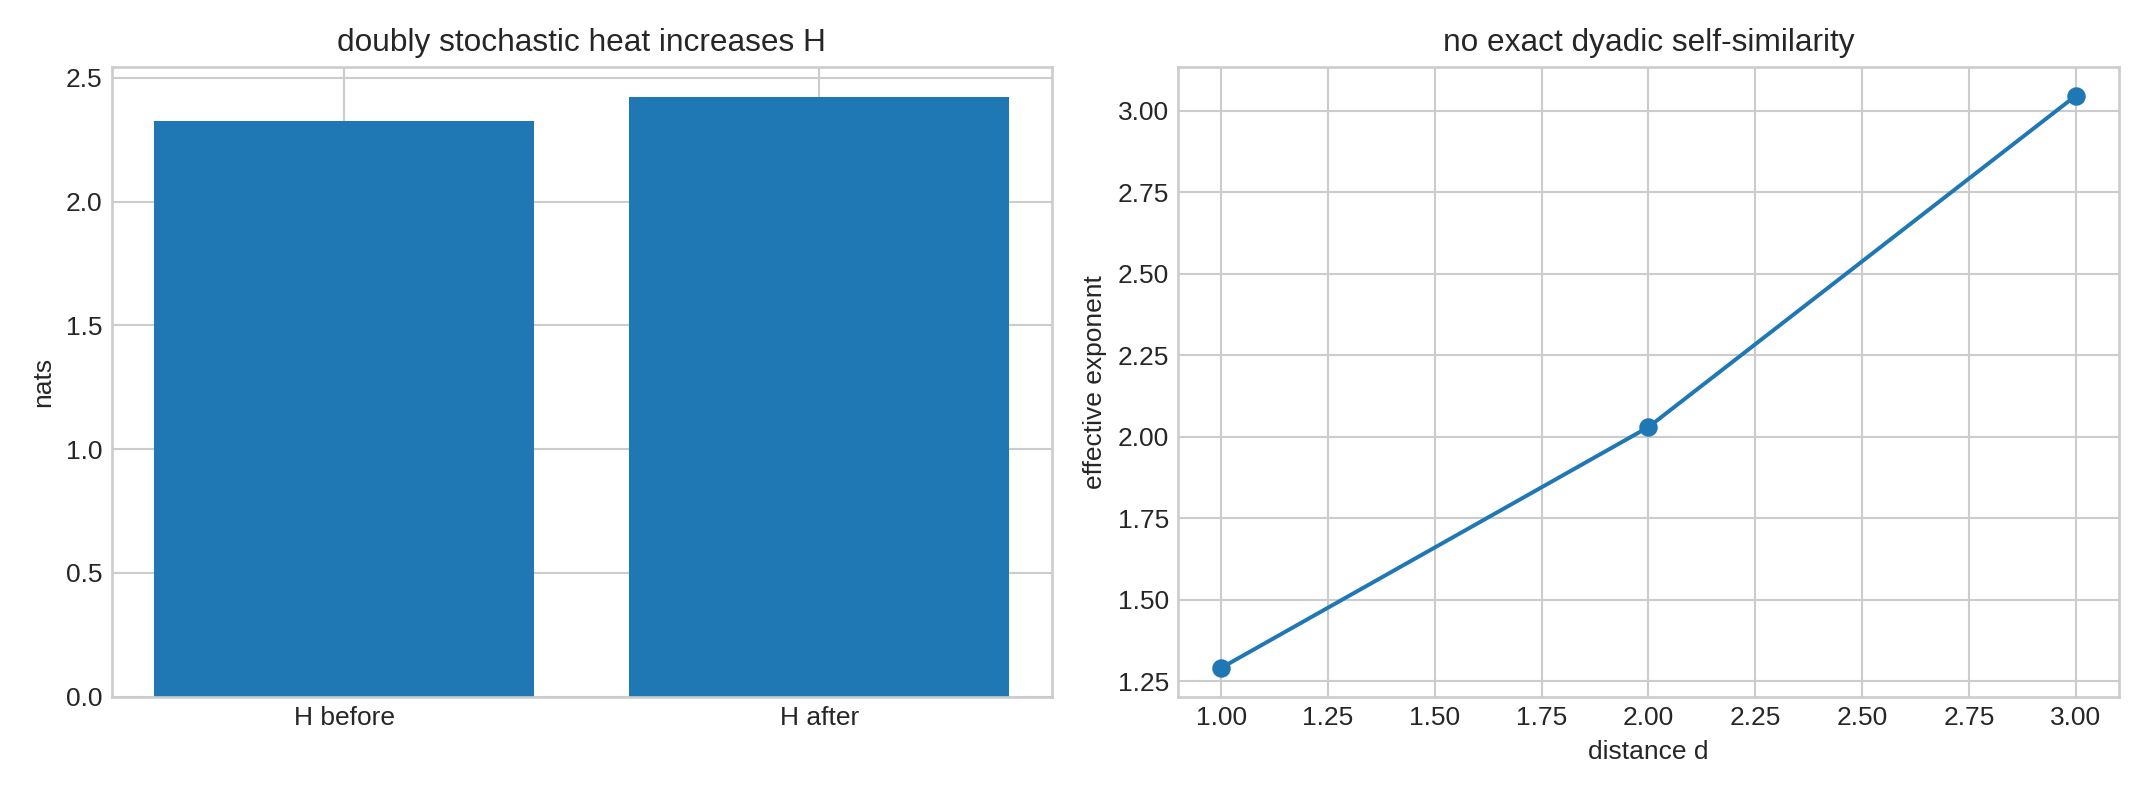
\includegraphics[width=0.96\textwidth]{FIN_ST46_ST57_Figures/st53_entropy_st56_compression.png}
\caption{Left: channel-specific entropy behavior. Right: the strict profile has no single dyadic ratio, and a coarse-only loss cannot select a refinement.}
\end{figure}

\statusboundary{} The quotient is a classification theorem. It establishes the precise meaning of information invariant under a change of faithful carrier; it does not prove that nature instantiates the groupoid. Thermodynamics still requires a bath or equilibrium family, a Hamiltonian/energy scale, temperature calibration, and an operational identification of heat and work. A dimensional constant cannot be manufactured from Shannon entropy alone.

\section{ST57 --- Minimal-axiom reconciliation}

The post-ST56 ledger retains nine source groups:
\begin{center}
\small
\begin{tabularx}{0.96\textwidth}{@{}l l X@{}}
\toprule
ID & Status & Reason\\
\midrule
A0 strict finite operator & retained & ST46 tightens its continuation but does not derive it\\
A1 state-selection event & retained & ST49 amplitude order is inserted\\
A2 refinement law & retained & ST47/ST56 require a scale or code law\\
A3 dimensional calibration & retained & ST53 information remains dimensionless\\
A4 operational process & constructible & ST55 packages but does not derive it from $A$\\
A5 external custody/data & retained & ST51/ST55 are local artifacts\\
A6 nonlinear response/gain & retained & ST48 proves gain-sign underdetermination\\
A7 connection/projective sector & conditional & ST49 inserts the $\pi$ texture\\
A8 temporal memory realization & retained & ST46 does not identify unique temporal completion\\
\bottomrule
\end{tabularx}
\end{center}

Three objects compress multiple obligations: the projective spinor packages A1, A7, and algebra completion; the two-carrier packet packages A4 and a record schema; the saturating order parameter packages A6 and a stable phase orbit. But packaging is not derivation. Removal countermodels keep the nine source groups independent relative to the present targets and construction classes.

\begin{theorem}[No strict axiom reduction in ST46--ST57]
No source group can be removed from the present physical-completion ledger on the strength of ST46--ST57. Conditional multi-obligation objects reduce bookkeeping only after their added premises are accepted.
\end{theorem}

\section{Falsification ledger and present interpretation}

The most informative results are not all positive:
\begin{itemize}
\item \textbf{Feedback falsification.} Equation~\eqref{eq:gain-family} proves that static symmetry and the strict fixed point do not identify positive gain.
\item \textbf{Refinement falsification.} Coarse intertwining and a coarse reconstruction loss leave the fine parameter free. Trace conservation chooses only after a new scale law is supplied.
\item \textbf{Naive fractality falsification.} The three exact-decimal dyadic profile ratios are interval-separated; no single amplitude rescaling describes them.
\item \textbf{One-component closure escape.} ST49 genuinely escapes ST38 by changing the state type. Its success is conditional and therefore locates, rather than removes, the missing premise.
\item \textbf{Dynamic equivalence falsification.} Five functions of one operator need not be similar as channels.
\item \textbf{Soliton falsification.} The completed ST34 saturation has an exactly uniform ground-state orbit, not a localized object.
\item \textbf{Thermodynamic falsification.} Data processing and entropy increase do not supply energy, temperature, or heat.
\end{itemize}

The deepest interpretation surviving this batch is therefore an \emph{operational spectral information framework with unresolved source laws}. The strict operator organizes multiple finite channels and supports exact data-processing statements. An enlarged projective state can carry topological and algebraic structure. But the choice of that state, the sign of adaptive feedback, the scale-refinement law, dimensional calibration, and the physical operational realization remain independent inputs.

This conclusion is compatible with the internal ontology in which the nadsoliton is primordial fractal information in a solitonic state. It is not a proof of that ontology. The mathematics currently establishes a candidate representational architecture, not the physical existence or uniqueness of the proposed primordial object.

\section{Recommended next programs ST58--ST69}

\small
\begin{longtable}{@{}p{0.08\textwidth}p{0.10\textwidth}p{0.74\textwidth}@{}}
\toprule
Program & Priority & Research test\\
\midrule
\endfirsthead
\toprule
Program & Priority & Research test\\
\midrule
\endhead
ST58 & 1 & Replace ST46 binary64 perturbation propagation by complete directed-interval eigenprojector, memory, inverse, and nonlinear-root evaluation.\\
ST59 & 2 & Search for one target-independent strict adaptive response functional and certify or refute positive reflection-odd gain.\\
ST60 & 3 & Derive or obstruct the ST49 projective spinor texture from the strict spectral bundle without choosing an origin label.\\
ST61 & 4 & Test whether a sourced trace or compression code can imply the ST47 trace-stationary law rather than merely assume it.\\
ST62 & 5 & Derive exact finite-count power bounds and minimum event counts for the ST51 transfer test.\\
ST63 & 6 & Classify completely positive operational intertwiners, not only matrix intertwiners between spectral images.\\
ST64 & 7 & Prove the minimal bath, scale, and equilibrium assumptions needed to convert the ST53 information ledger into thermodynamics.\\
ST65 & 8 & Prove nonexistence of localized stationary states or interval-certify a localized excited orbit in the ST34 saturation.\\
ST66 & 9 & Replace the illustrative polar flow by a smooth polynomial $C_{12}$-equivariant multi-component bifurcation and classify its branches.\\
ST67 & 10 & Separate $\pi$ holonomy from chirality and test one genuinely orientation-sensitive projective invariant.\\
ST68 & 11 & Add calibration uncertainty, event validation, and independent-custody requirements to the ST55 executable specification.\\
ST69 & 12 & Recompute the axiom graph after ST58--ST68 and test whether any conditional package becomes strict-sourced.\\
\bottomrule
\end{longtable}
\normalsize

The recommended order is deliberately proof-first: ST58 closes a known arithmetic gap; ST59 and ST60 attack the two highest-value missing sources; ST61 tests the claimed fractal-compression route; and ST62--ST68 strengthen operational and nonlinear consequences without confusing them with external validation.

\section{Reproducibility and audit boundary}

The release packet contains:
\begin{itemize}
\item \texttt{fin\_st46\_st57\_research.py} --- deterministic analysis and figure generation;
\item \texttt{test\_fin\_st46\_st57.py} --- seventeen live acceptance tests;
\item \texttt{FIN\_ST46\_ST57\_Results.json} and \texttt{FIN\_ST46\_ST57\_Summary.csv};
\item the ST46 sensitivity certificate, ST51 preregistration, and ST55 executable specification;
\item seven generated figures and a SHA-256 release manifest.
\end{itemize}

The random seed is 20260813. The numerical environment and dependency versions are serialized in the result ledger. The full test command is
\[
\texttt{python3 -m unittest -v test\_fin\_st46\_st57.py}.
\]
All seventeen tests passed in the release replay.

The code and tests verify internal consistency, hashes, exact rational brackets, live projective holonomy, finite intertwiner dimensions, synthetic receiver behavior, entropy inequalities, and refinement nonselection. They cannot provide external custody, apparatus calibration, physical dimensions, or laboratory data.

\section{Final conclusion}

ST46--ST57 sharpen rather than overturn the current FIN state map.

\begin{enumerate}
\item The collision mechanism remains numerically robust under conservative upstream sensitivity, but one final all-directed interval replay is still required.
\item A refinement can be selected only after a scale or code principle is supplied; neither ordinary coherence nor the tested coarse compression criterion supplies it.
\item Positive feedback is not a consequence of the strict static operator and symmetry alone.
\item A projective two-component state is the smallest successful object found here that can package selector data, full algebra, and nontrivial holonomy. Its origin remains the central missing theorem.
\item Carrier-neutral information is rigorously the operational-isomorphism class of a complete experiment, not a spectrum and not information without realization.
\item The strict heat and unitary channels support valid information-theoretic statements, but no thermodynamic or dimensional bridge follows without additional physical structure.
\item The constructed saturating nonlinear model is rigorously stable but spatially uniform; it does not derive matter or a localized particle.
\end{enumerate}

Accordingly, the batch produces a genuine new theoretical object and several proof-grade obstructions, but no strict selector closure, dimensional physics, legacy-role transfer, experimentally validated carrier equivalence, Standard Model, gravity, or Theory-of-Everything theorem.

\vfill
\begin{center}
\small
Release 10.58 --- English research report --- CC BY 4.0
\end{center}

\end{document}
